Despite Open-Source Software being popular, widely used and implemented in production, there's no definite consent regarding the ideal and most favoured release frequency and size. Some projects release several times per month while the others only once per quarter or even less. Also releases differ in size, number of commits and fixed issues they address. My goal is to explore some potential hidden patterns which could be generalized and used in the future release planning and policy in Open-Source space.\\
Another issue and not only with Open-Source projects are bugs and finding workarounds and temporary solutions for them. We all know the scenario when a correct code doesn't function properly. We head to Stack Overflow or Reddit and start to look for similar problems. If lucky enough, we find a question with a solution presented in the comment section. But that's not always the case. Especially questions about faults caused by library/framework bugs have often empty and not really helpful comment sections because there should not be such problem in the first place. Such situations can eat up a lot of developers' time and kill productivity. Therefore I hoped to create an algorithm which could link corresponding GitHub and Stack Overflow items and make these frustrating situations easier.

This thesis is divided into 2 parts. I aimed to create a framework which could be potentially used as a base of tool used to recognize level of user satisfaction and its sudden changes. Second part of the framework should be able to find and link pairs of issues reported in bug tracking systems and their respective social media entries. Both parts of the framework use various text processing methods, sentiment analysis concentrating more on machine learning while bug linking utilizes topic modelling and text similarity concepts.\\
\begin{figure}%
    \centering
	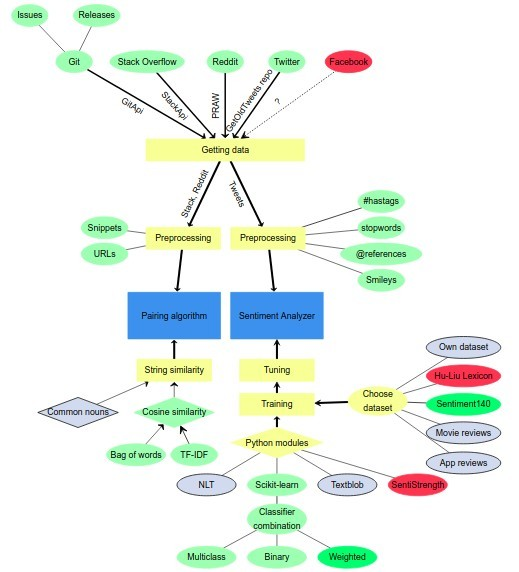
\includegraphics[width=15cm]{dataflow_final_yed.jpg}
    \caption{Brief sketch of dataflow in the proposed framework}%
    \label{fig:frameworkDataflow}%
\end{figure}
As can be seen in Figure \ref{fig:frameworkDataflow}, two final products of the framework are sentiment classifier and linking algorithm. Green elements are the ones used in final solution, grey ones were tested and considered and red ones were left out or not possible to implement. Work on the framework could be divided into several steps:
\begin{enumerate}
\item{\textbf{Getting the data} - there is no data science, machine learning or natural language processing without the data. That is why the very first step is to create a mechanism to easily mine data from various sources. Git mining is required to get information about OSS projects and is described in subsections number \ref{ssec:gitReleaseDatesMining} and \ref{ssec:issuesMining} while Twitter, Reddit and SO were mined to provide data which are the target of analysis \ref{ssec:GettingData}.}
\item{\textbf{Data preprocessing} - all textual information, especially those which originate on social media contain noise. To get rid of all this extra information, which might cause inaccuracies and faults, data preprocessing is a necessary step.}
\item{\textbf{Finding a right training dataset} - since the performance of any ML algorithm is very tightly bound to the training data used, this step should not be neglected and be considered as important step as any other. It is described in the Section \ref{sec:trainingDatasets}.}
\item{\textbf{Choosing a tool/module/library and particular classification algorithm} - there are many algorithms used for classification but environment for their usage and best performance differs greatly. To choose a correct algorithm and find the best combination of parameter values is often a long process. Things do not get any easier when we take into account that there are not only many algorithms but they are actually also implemented in several programming languages and libraries. Inconsistencies between results of several SE modules were pointed out by Bin Li at al. in his paper \textit{How far can we go}. My approach to problems and challenges of this step are described in great detail in sections number \ref{sec:languageProcessingTools} and \ref{sec:classifierEvaluation}}
\item{\textbf{Topic modeling and text similarity} - this is the crucial step for the second part of the framework. Once the data are downloaded from Git as well as from social media, the last step to do is to find the matches.   This part is described in Chapter \ref{chap:pairingBugs}.}
\end{enumerate}
After all the steps are implemented, proposed framework will be completed. But that does not guarantee that the output data are easy to interpret. That's why one extra additional step is needed. Using some statistics and data science methods, I am interpreting the results in Subsection \ref{ssec:crossCorrelation} and Subsection \ref{ssec:crossCorrelationCommits}.

\newpage
\textbf{This framework targets following research questions:}
\begin{itemize}
\item{\textbf{$RQ_{1}$}: Do the OSS projects which release more often get general better sentiment score on social media?}
\item{\textbf{$RQ_{2}$}: Does a release have an immediate effect on sentiment?}
\item{\textbf{$RQ_{3}$}: Is there a correlation between sentiment change and size of the release (number of commits) ?}
\item{\textbf{$RQ_{4}$}: Is it possible to link social media entries to their respective bugs which they talk about?}
\end{itemize}